\documentclass[12pt, a4paper, openany]{report}

\def\VersionRapport{1.0}

\usepackage[utf8]{inputenc} % un package
\usepackage[T1]{fontenc}      % un second package
\usepackage[francais]{babel}  % un troisième package
\usepackage{layout}
\usepackage[top=2.7cm, bottom=2.5cm, left=3.5cm, right=3cm]{geometry}
\usepackage{setspace}

\frenchbsetup{StandardLists=true} % à inclure si on utilise \usepackage[french]{babel}
%\usepackage{enumitem}
\usepackage[shortlabels]{enumitem}
\usepackage{amssymb}

\usepackage{color}
\usepackage{listings}
\definecolor{dkgreen}{rgb}{0,0.6,0}
\definecolor{gray}{rgb}{0.5,0.5,0.5}
\definecolor{mauve}{rgb}{0.58,0,0.82}

\lstset{frame=tb,
  language=Matlab,
  aboveskip=3mm,
  belowskip=3mm,
  showstringspaces=false,
  columns=flexible,
  basicstyle={\small\ttfamily},
  keywordstyle=\color{blue},
  commentstyle=\color{dkgreen},
  stringstyle=\color{mauve},
  breaklines=true,
  breakatwhitespace=true,
  tabsize=3,
  breaklines=true,
  morekeywords={matlab2tikz},
  morekeywords=[2]{1}, 
  keywordstyle=[2]{\color{black}},
  identifierstyle=\color{black},
  numbers=left,
  numberstyle={\tiny \color{black}},
  numbersep=9pt, 
  emph=[1]{for,end,break},
  emphstyle=[1]\color{red}
}

\usepackage{multirow} % pour les tableaux
\usepackage[table]{xcolor} % pour les tableaux

\usepackage{verbatim}
\usepackage{moreverb}
\usepackage{url}
\usepackage{pst-all}
\usepackage{eso-pic,graphicx}
\usepackage{caption} 
\usepackage[colorlinks=true,urlcolor=blue,linkcolor=red]{hyperref}
\usepackage{array}
\usepackage[toc,page]{appendix}
\usepackage[off]{auto-pst-pdf}
\usepackage{hyperref} % pour le sommaire table des matières
\AddThinSpaceBeforeFootnotes % à insérer si on utilise \usepackage[french]{babel}
\FrenchFootnotes % à insérer si on utilise \usepackage[french]{babel}
\usepackage{fancyhdr}
\pagestyle{headings}
\usepackage{pifont}  %pour les puces
\usepackage{amsmath} %pour les puces

\usepackage{verbatim} % pour le code en annexe 

%%%%%%%colones 
\newcolumntype{R}[1]{>{\raggedleft\arraybackslash }b{#1}}
\newcolumntype{L}[1]{>{\raggedright\arraybackslash }b{#1}}
\newcolumntype{C}[1]{>{\centering\arraybackslash }b{#1}}
%%%%%%% 

\renewcommand{\appendixpagename}{Annexes}
\renewcommand{\appendixtocname}{Annexes}

\title{Theme: Compte Rendu Système Linéaire à Temps Continu 1}
\author{REBOUT \bsc{Mehenna}}
\author{BOUYOUCEF \bsc{Farid}}
\date{2018-2019}



%new
\newcommand{\HRule}{\rule{\linewidth}{0.5mm}}


\begin{document}

%\selectlanguage{francais}
\pagenumbering{arabic} 

\makeatletter
  \begin{titlepage}
  

  \begin{sffamily}
   \begin{center}

    % Upper part of the page. The '~' is needed because \\
    % only works if a paragraph has started.
    
\includegraphics[scale=0.5]{Logo_UT3.jpg}~\\[1.5cm]

    \textsc{\LARGE Master 1 EEA ISTR/RODECO  }\\[2cm]

    \textsc{\Large Compte Rendu  Système Linéaire à Temps Continu 1}\\[1.5cm]

    % Title
    \HRule \\[0.4cm] % saut de ligne
    { \huge \bfseries TP 1 Pendule\\[0.4cm] }

    \HRule \\[1cm]   % sous de ligne 
    
\includegraphics[scale=0.1]{logomaster.jpg}
    \\[1cm]

    % Author and supervisor
    \begin{minipage}{0.4\textwidth}
      \begin{flushleft} \large
         \textsc{\emph {Réalisés par:} \\REBOUT Mehenna}\\
         \textsc{BOUYOUCEF Farid}   
          \newline
          Promotion 2018-2019 \\
      \end{flushleft}
    \end{minipage}
    \begin{minipage}{0.4\textwidth}
      \begin{flushright} \large
        \emph{Tuteur :}  \textsc{M DUROLA}\\
        \emph{Responsable de la Formation:} \textsc{M GOUAISBAUT}
      \end{flushright}
    \end{minipage}

    \vfill

    % Bottom of the page
    {\large Octobre 2018}

  \end{center}
  \end{sffamily}      
          
  \end{titlepage}
  
\makeatother




   
%*********************** somaire **************
\renewcommand{\contentsname}{Sommaire}
\tableofcontents
%*********************** listes des figures **************
\listoffigures
%*********************** listes des tableaux **************
\listoftables



%*********************** INTRODUCTION **************
\chapter*{Introduction}
\addcontentsline{toc}{chapter}{Introduction}

\paragraph{Présentation du pendule inversé :} La Figure 1 donne une représentation schématique du pendule. Le bras est relié au moteur, qui entraîne la rotation du bras et donc du pendule. Il a une longueur L{r} et un moment d'inertie J{r} . Nous noterons son angle $\theta$ . Le pendule, quant à lui, est axé au bout du bras. Il a une longueur L{p}. Son moment d'inertie au centre de masse est noté J{p}. On note l'angle que fait l'axe du pendule avec l'axe verticale a (en radian).

\begin{center}
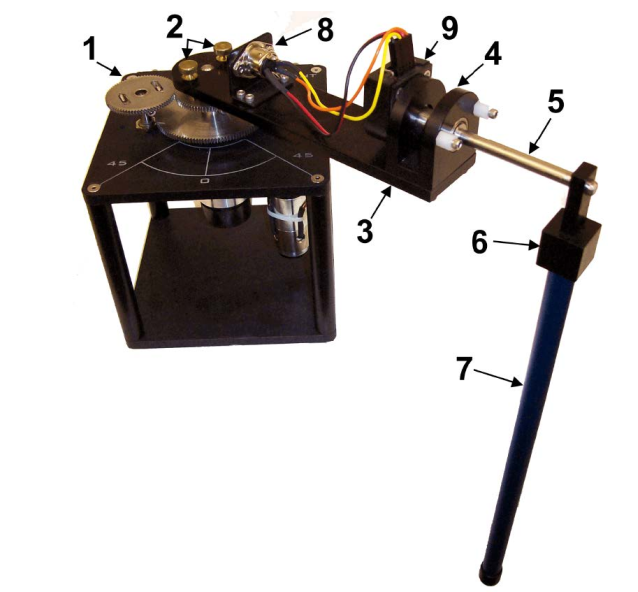
\includegraphics[scale=0.5]{pondule.png}
\captionof{figure}{\textit{Composant du pendule}}
\label{fig1} 
\end{center}

\paragraph{Précision du lieu :} Ce TP a eu lieux a l’université Paul SABATIER dans la salle TP I3.   

\paragraph{La date :} Ce sujet nous a été attribué par M DUROLA le mois d'octobre  et on va le rendre le 19/11/2018 à M DUROLA.

\paragraph{But de la manipulation :}  Dans cette manipulation on se propose de réaliser un asservissement permettant la régulation du pendule inversé représentée par la Figure 1.1 en position haute comme le montre la Figure 1.2. On utilisera pour cela les techniques d'espace d'état à temps continu. Cette manipulation est constituée de quatre grandes étapes : modélisation, analyse, régulation et implémentation. Les objectifs du TP sont les suivants :
\begin{itemize}
\item Savoir établir un modèle linéarisé autour d'un point d'équilibre.
\item Savoir établir les propriétés structurelle d'un système linéaire.
\item Savoir utiliser Matlab et sa toolbox simulink.
\item Savoir synthétiser une commande par retour d'état.
\item Savoir faire la simulation de modèles linéaires et non linéaires.
\item Savoir utiliser les différentes commandes MATLAB pour étudier un système.

\end{itemize}

    
    %******************* MODÉLISATION **********
 \chapter{Modélisation}
 
 La Figure 1.1 donne une représentation schématique du pendule. Le bras est relié au moteur, qui entraîne la rotation du bras et donc du pendule. Il a une longueur $L_{r}$ et un moment d'inertie $J_{r}$. Nous noterons son angle $\theta$.\\
 Le pendule, quant à lui, est lixé au bout du bras. Il a une longueur $L_{p}$ . Son moment d'inertie au
centre de masse est noté $J_{p}$. On note l'angle que fait l'axe du pendule avec l'axe verticale $\alpha$ (en radian).\\
 Tous les calculs de la modélisation se feront en prenant pour origine, la position haute du pendule. pour les descriptions et les valeurs numériques des constantes se reporter à la Table \ref{table12}\\
 

\begin{center}
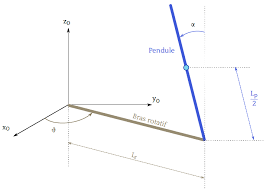
\includegraphics[scale=1]{ShemaPendule.png}
\captionof{figure}{\textit{Schéma du pendule rotatif.}}
\label{fig2} 
\end{center}


\begin{center}
\begin{tabular}{|l|c|}
\hline \rowcolor{mauve} $N^{0}$ & Composant\\
\hline 1 & SRV02\\
\hline 2 & Vis\\
\hline 3 & Bras\\
\hline 4 & Logement d’arbre\\
\hline 5 & Arbre\\
\hline 6 & Raccord\\
\hline 7 & Pendule\\
\hline 8 & Connecteur de l'encodeur\\
\hline 9 & Encodeur\\
\hline
\end{tabular}

\captionof{table}{\textit{Nomenclature des composants de la maquette.}}
\end{center}

     

\begin{center}
\begin{tabular}{|l|c|r|}
\hline \rowcolor{mauve} Symbole & Description &  Valeur  \\
\hline $B_{p}$  &  Coef de frottement visqueux du pendule  & $0.0024 kg/m^{2}$   \\
\hline $B_{r}$ & Coef de frottement visqueux du bras & $0.0024 kg/m^{2}$ \\
\hline $\eta_{g}$  &  Rendement du réducteur  & $0.9$  \\
\hline $\eta_{m}$  &  Rendement du moteur  & $0.69$  \\
\hline $K_{g}$  &  Rapport de vitesse  & $70$  \\
\hline $K_{m}$  &  Gain f.e.m  & $7.68\times10^{-3} V/(rad/s)$ \\
\hline $K_{t}$  &  Gain couple moteur/courant  & $7.68\times10^{-3} N.(m/A)$\\
\hline $J_{p}$ &  Moment d'inertie du pendule au ctr de masse & $0.0012 kg/m^{2}$ \\
\hline $J_{r}$  &  Moment d'inertie du bras au ctr de masse  & $9.98\times10^{-4} kg/m^{2}$ \\
\hline $L_{m}$  &   Inductance du moteur & $0.18 mH$\\
\hline $L_{p}$  &  longueur du pendule  & $0.337 m$ \\
\hline $L_{r}$  &  Inductance du bras, du pivot à l'extrémité   & $0.216 m$ \\
\hline $m_{p}$  &  Masse du pendule  & $0.127 kg$\\
\hline $m_{r}$  &   Masse du bras  & $0.257 kg$\\
\hline $R_{m}$  &   Résistance du moteur  & $2.60 \Omega$ \\
\hline $V_{m}$  &  Tension envoyé au moteur   &  A régler \\

\hline 
\end{tabular}
\captionof{table}{\textit{Liste des données spécifique au système}}
\label{table12}
\end{center} 

Les équations du mouvement, déterminées à l'aide de la mécanique Lagrangienne, sont données par les
deux équations différentielles suivantes : \\\\

$\bigg(m_{p}L_{r}^{2} + \frac{1}{4}m_{p}L_{p}^{2} - \frac{1}{4}m_{p}L_{p}^{2}cos(\alpha^{2}) + J_{r} \bigg)\ddot{\theta}- \bigg(\frac{1}{2}m_{p}L_{p}L_{r}\cos(\alpha) \bigg)\ddot{\alpha}+$\\  $\bigg(\frac{1}{2}m_{p}L_{p}^{2}\sin(\alpha)\cos(\alpha) \bigg)\dot{\theta}\dot{\alpha} + \bigg(\frac{1}{2}m_{p}L_{p}L_{r}\sin(\alpha) \bigg)\dot{\alpha}^{2}=\frac{\eta_{g}K_{g}\eta_{m}k_{t}(V_{m}- K_{g}k_{m}\dot{\theta})}{R_{m}}-B_{r}\dot{\theta}$ $\hspace{1mm}(1)$ \\\\\\\\ 

$-\frac{1}{2}m_{p}L_{p}L_{r}\cos(\alpha)\dot{\theta}+(J_{p}+\frac{1}{4}m_{p}L_{p}^{2})\ddot{\alpha}-\frac{1}{4}m_{p}L_{p}^{2}\cos(\alpha)\sin(\alpha)\dot{\theta}^{2}-\frac{1}{4}m_{p}L_{p}g\sin(\alpha)$\\$=-B_{p}\dot{\alpha}$   $\hspace{3mm}(2)$ \\\\\\
  
  %$\bigg(m_{p}L_{r}^{2} + \frac{1}{4}m_{p}L_{p}^{2} - \frac{1}{4}m_{p}L_{p}^{2}cos(\alpha^{2}) + J_{r} \bigg)$ $\ddot{\theta}$

   


\section{Étude succincte du modèle non linéaire  }

Dans un premier temps, nous allons étudier le modèle non linéaire représenté par les deux équations (1),(2) du mouvent.

 \paragraph{Proposition des variables d'état :\\}

 On propose quatre variables d'état : \\
 soit : $\alpha$, $\dot{\alpha}$ et  $\theta$, $\dot{\theta}$\\
 
 \paragraph{Les points d'équilibre en fonction de $V_{m}$ :\\}
 
 si on prend  $V_{m}=0$ donc y a une infinité des points d'équilibre \\
 alors que si on prend $V_{m}=$constante   .... bla bla \\
 
  \paragraph{Simulation du dispositif non linéaire aux points d'équilibre :\\}
 
  
\begin{center}
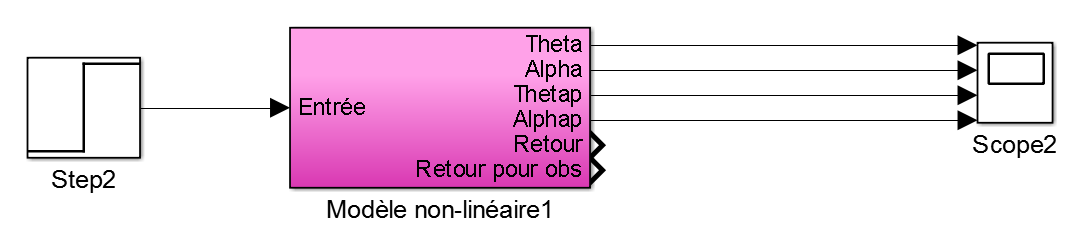
\includegraphics[scale=0.5]{modelenonlineairesimulink.png}
\captionof{figure}{\textit{simulation du dispositif non linéaire.}}
\label{fig1} 
\end{center} 
 
 ilaq aliii il me manque la figure ..... \\\\\\\\\\\\\\
 
 \paragraph{Simulation pour des condition initiales :\\} 
 
 pour les premiers conditions soit :\\
$\alpha=+1$; $\theta=0$; $\dot{\alpha}=0$; $\dot{\theta} = 0:$ \\
                                                   
\begin{center}
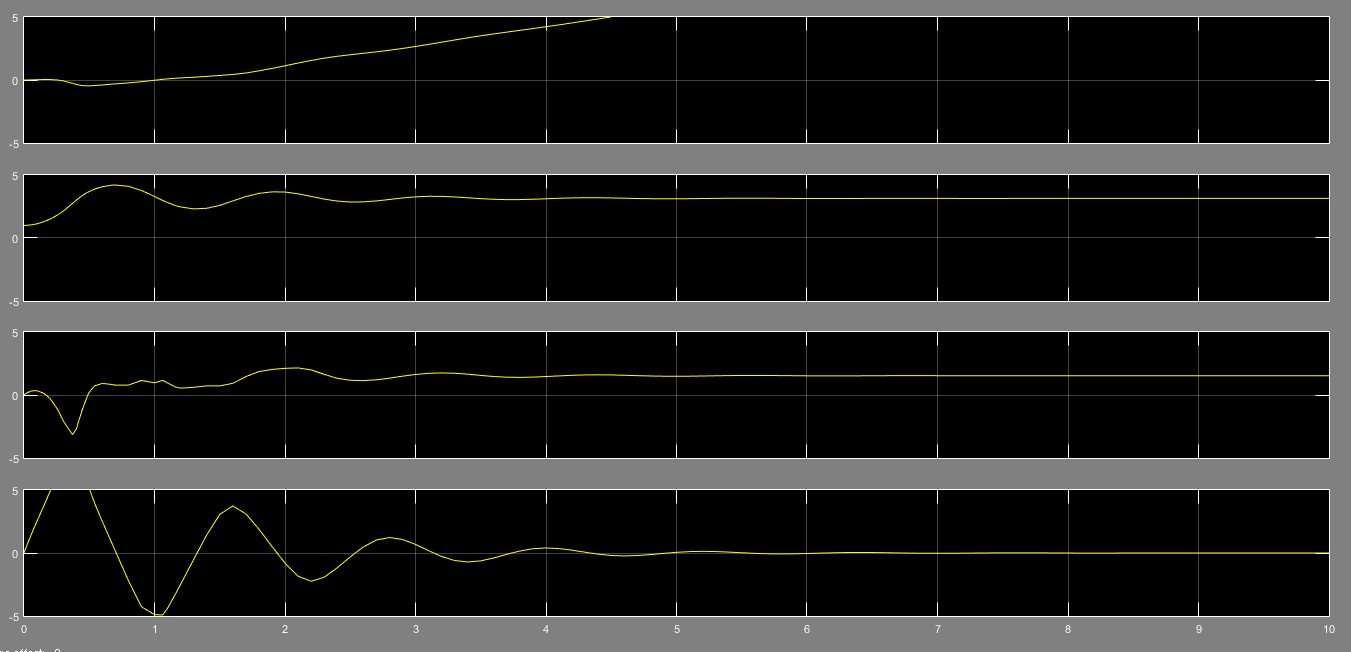
\includegraphics[scale=0.4]{alpha=+1.PNG}
\captionof{figure}{\textit{simulation $\alpha=+1$.\\}}
\label{fig1} 
\end{center}
 
D’après la figure 1.3 on remarquant que $\alpha$ tend vers $\pi$ et $\theta$
tend vers l'infini, ce qui ne donne un bruit, on souhaite alors d'avoir $\theta$ qui varié peut ou bien d'avoir $\theta$=cste.\\\\  
 
et pour les deuxièmes conditions soit :\\
$\alpha=-1$; $\theta=0$; $\dot{\alpha}=0$; $\dot{\theta} = 0:$ \\
                                                   
\begin{center}
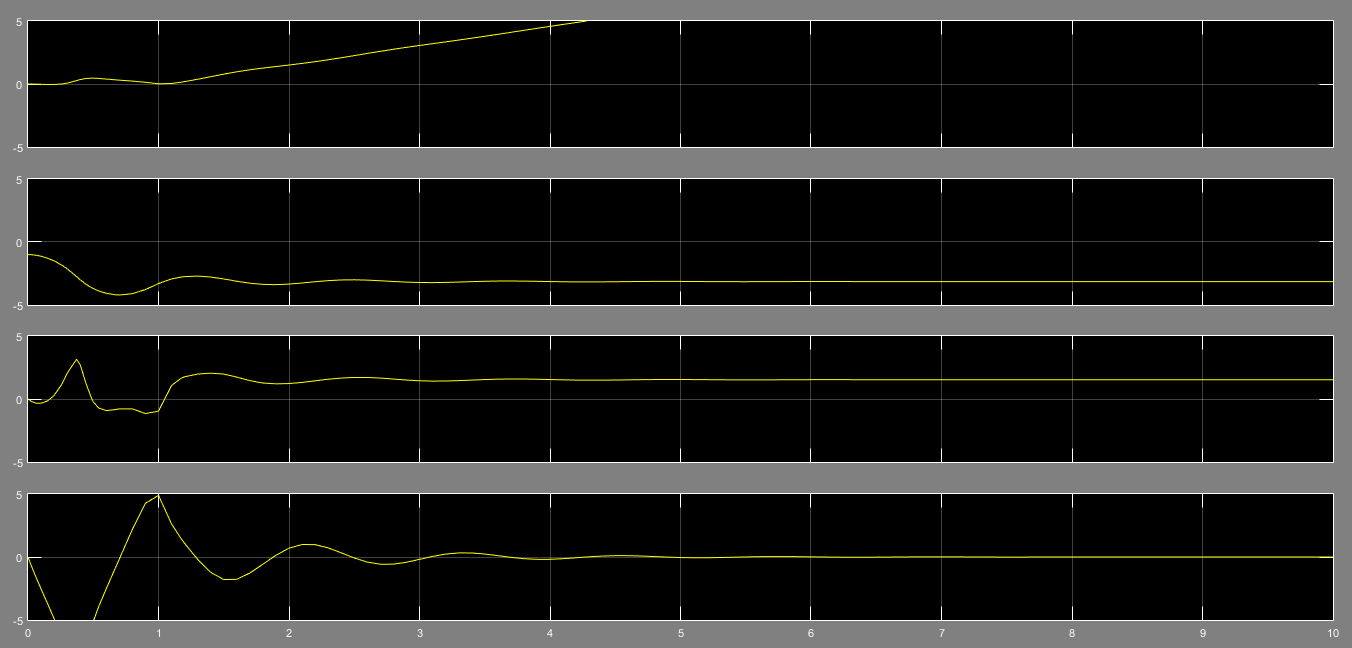
\includegraphics[scale=0.4]{alpha=-1.PNG}
\captionof{figure}{\textit{simulation $\alpha=-1$.\\}}
\label{fig1} 
\end{center}

D’après la figure 1.4 on remarquant que $\alpha$ tend vers $-\pi$ et de même pour $\theta$
tend vers l'infini, ce qui ne donne un bruit, on souhaite alors d'avoir aussi $\theta$ qui varié peut ou bien d'avoir $\theta$=cste, \hyperref[section1.1]{voir Annexe 1}\label{annexe1}.\\\\

\section{Linéarisation et obtention d'un modèle linéaire}
\paragraph{Linéarisation du système non linéaire :\\}
Dans cette partie on a choisit comme variable d'état :

 $x(t)=\bigg[\theta(t)\hspace{3mm}\alpha(t)\hspace{3mm} \dot{\theta}(t)\hspace{3mm} \dot{\alpha}(t)\bigg]^{T}$ \\  
   et à cet effet on utilise une décomposition en série de Taylor arrêtée à l'ordre 1 :\\
   
   $\tilde{f}(z)=f(z_{o})+\left.\begin{matrix}\sum_{i=1}^{n}\frac{\partial f }{\partial zi}\end{matrix}\right|_{z_0} (z_{i}-z_{o})$ \\\\ 
   
   %%%%%%%%%%%%%%%%%%%%%%%%%%%%%%%%%%%%%%%%%%%%%%%%%%%%%%%%%%%
   On cherche a avoir des équations en fonction de:  $\ddot{\theta }$, $\ddot{\alpha}$, $\dot{\alpha}$ et $\dot{\theta}$. On va isoler d'abord $\ddot{\theta }\:$ et ensuite $\ddot{\alpha}$.

D'après l'équation (1) du Chapitre 1, on a : \\


    $E\ddot{\theta }-F\ddot{\alpha}+ G\dot{\alpha}\dot{\theta}+H\dot{\alpha}^2=IV_{m}-IK_{g}K_{m}\dot{\theta}-B_{r}\dot{\theta}$\\\\

et aussi d'après l'équation (2) du Chapitre 1, on a :\\ 


$-{E}'\ddot{\theta}+{F}'\ddot{\alpha}-{G}'\dot{\theta}^2-{H}'=-B_{p}\dot{\alpha}$ \\\\

avec: \\

$E=(m_{p}{L_{r}}^2+\frac{1}{4}m_{p}{L_{p}}^2-\frac{1}{4}m_{p}{L_{p}}^2cos({\alpha})^2+Jr)$ \\

$F=(\frac{1}{2}m_{p}L_{p}L_{r}cos(\alpha))$\\

$G(\frac{1}{2}m_{p}{L_{p}}^2sin(\alpha)cos(\alpha))$\\

$H=(\frac{1}{2}m_{p}L_{p}L_{r}sin(\alpha))$\\

$I=(\frac{\eta_{g}K_{g}\eta_{m}k_{t}}{R_{m}})$\\

${E}'=(\frac{1}{2}m_{p}L_{p}L_{r}cos(\alpha))$\\

${F}'=(J_{p}+\frac{1}{4}m_{p}{L_{p}}^2)$\\

${G}'=(\frac{1}{2}m_{p}{L_{p}}^2sin(\alpha)cos(\alpha))$\\

${H}'=(\frac{1}{2}m_{p}L_{p}L_{r}gsin(\alpha))$\\\\

et on va extraire $\ddot{\theta }$ et $\ddot{\alpha}$ et on obtient :\\

 $\ddot{\theta }=\frac{1}{E}(F\ddot{\alpha}-G\dot{\alpha}\dot{\theta}-H\dot{\alpha}^2+IV_{m}-IK_{g}K_{m}\dot{\theta}-B_{r}\dot{\theta})$\\\\
   ainsi :
   $\ddot{\alpha}=\frac{1}{{F}'}({E}'\ddot{\theta}+{G}'\dot{\theta}^2+{H}'-B_{p}\dot{\alpha})$ \\


 Premièrement, on remplace $\ddot{\alpha}$ dans l'équation de $\ddot{\theta}$ et on obtient :\\ 


$\ddot{\theta}=\frac{1}{E{F}'-F{E}'}(F{G}'\dot{\theta}^2+F{H}'-FB_{p}\dot{\alpha}-G{F}'\dot{\alpha}\dot{\theta}-H{F}'\dot{\alpha}^2+I{F}'V_{m}-{F}'IK_{g}K_{m}\dot{\theta}$\\$-{F}'B_{r}\dot{\theta})$\\ 

D'où :\\

$J_{t} = E{F}'-F{E}'$\\\\ $=(m_{p}{L_{r}}^2+\frac{1}{4}m_{p}{L_{p}}^2-\frac{1}{4}m_{p}{L_{p}}^2cos({\alpha})^2+Jr)(J_{p}+\frac{1}{4}m_{p}{L_{p}}^2)$\\
$-\frac{1}{2}m_{p}L_{p}L_{r}cos(\alpha))(\frac{1}{2}m_{p}L_{p}L_{r}cos(\alpha))$\\\\


Après avoir réaliser les simplification et aussi on pose :  $cos(\alpha)=1$ , on obtient alors \\


     $J_{t}=J_{p}m_{p}{L_{p}}^2+J_{p}J_{r}+\frac{1}{4}m_{p}{L_{p}}^2J_{r}$\\\\


 En suite, on remplace $\ddot{\theta}$ dans l'équation de $\ddot{\alpha}$ et on obtient :\\

    $\ddot{\alpha}=\frac{1}{E{F}'-F{E}'}(-{E}'G\dot{\alpha}\dot{\theta}-{E}'H\dot{\alpha}^2+{E}'IV_{m}-{E}'IK_{g}K_{m}\dot{\theta}+{E}'B_{r}\dot{\theta}+E{G}'\dot{\theta}^2+E{H}'$\\$-EB_{p}\dot{\alpha})$\\\\


On dérivant, et on va construire la matrice $A_{haut}$ et le vecteur $B_{haut}$.\\
On pose alors :\\

$\alpha = 0 \Rightarrow \hspace{3mm} cos(\alpha) = 1$ et $sin(\alpha) = 0$ 


\begin{equation*}
\left\{\begin{matrix}
\dot{x}(t) = \begin{bmatrix}
\dot{\theta}(t)\\ 
\dot{\alpha}(t)\\ 
\ddot{\theta}(t)\\ 
\ddot{\alpha}(t)
\end{bmatrix} = A_{haut}*\begin{bmatrix}
\theta(t)\\ 
\alpha(t)\\ 
\dot{\theta}(t)\\ 
\dot{\alpha}(t)
\end{bmatrix} + B_{haut} V_m\\ 

Avec : \dot{x_1}(t) = x_3(t) = \dot{\theta}\; et \; \dot{x_2}(t) = x_4(t) = \dot{\alpha}
\end{matrix}\right.
\end{equation*}

D’où : 
\begin{equation*}
    A_{haut} = \frac{1}{J_t} \begin{bmatrix}
0 & 0 & J_t & 0\\
0 & 0 & 0 & J_t\\
0 & \frac{1}{4}{m_p}^2{L_p}^2L_rg & F'(-B_r-K_gK_mI)& -FB_p \\
0 & \frac{1}{2}m_pL_pg(J_r+m_p{L_r}^2) & E'(B_r-K_gK_mI) & -EB_p\\
\end{bmatrix}
\end{equation*}

\begin{equation*}
    B_{haut} = \begin{bmatrix}
    0\\ 
    0\\ 
    F'I\\ 
    E'I
\end{bmatrix}
\end{equation*}

On remplace alors E,F,I,E',F' par leurs expressions que on a supposer au dessus, et on obtient : 
\begin{equation*}
    A_{haut} = \frac{1}{J_t} \begin{bmatrix}
0 & 0 & J_t & 0\\
0 & 0 & 0 & J_t\\
0 & \frac{1}{4}{m_p}^2{L_p}^2L_rg & (J_p+\frac{1}{4}m_p{L_p}^2)(-B_r-K_gK_m\gamma)& -\frac{1}{2}m_pL_pL_rB_p \\
0 & \frac{1}{2}m_pL_pg(J_r+m_p{L_r}^2) & (\frac{1}{2}m_pL_pL_r)(B_r-K_gK_m\gamma) & -(J_r+m_p{L_r}^2)B_p\\
\end{bmatrix}
\end{equation*}

\begin{equation*}
    B_{haut} = \begin{bmatrix}
    0\\ 
    0\\ 
    (J_p+ \frac{1}{4}m_p{L_p}^2)\gamma\\ 
    \frac{1}{2}m_pL_pL_r\gamma
\end{bmatrix}
\end{equation*}


\paragraph{Simulation de la réponse à des conditions initiales :\\}


ilaq les figure ni .....



%%%%%%%%%%%%%%%%%%%%%%%%%%%%%%%%%%%%%%%




 %\begin{enumerate}[(a)]
  % \item Le système sera stable en boucle fermée
   %\item Une erreur de position nulle
   %\item Une erreur de vitesse limitée à 1 i.e. lorsque l'entrée de consigne est une rampe de pente 1
   %\item Une convergence vers la consigne en moins de 3 seconde, sans oscillations, ni dépassement.
   %ù\item Un rejet de la perturbation de fuite.
   %ù\item Un rejet du bruit de mesure au-delà de 100 Hz d’au moins de 60 dB par.
 %\end{enumerate}
	
%*********************** Problématique **************
\chapter{Analyse temporelle et structurelle du modèle linéarisé }
 %\chaptermark{Cmd proportionnelle intégrales} (pour avoir ce titre en petit 
\section{Analyse de la stabilité asymptotique du point d'équilibre haut}





 
 
 
 
 
 %%%%%%%%%%%%%%%%%%%%%%bouyoucef%%%%%%%%%%%%%%%
\chapter{RÉGULATION DU MODÈLE LINÉARISÉ}

     \section{Schéma de loi de commande permettant de placer les valeurs propres du système bouclé en}
  $p=
  \begin{bmatrix}
  -108&-0.3&-4.3+2.2i&-4.3-2.2i
  \end{bmatrix}^{T}$\\
  
  
   Les pôles a partie  réelles négatives nous permet d'avoir un système stable .\\

   La convergence vers le point d’équilibre est  assuré a l'aide des partie imaginaire des pôles,le pôles    le plus grande nous as permet d’augmenter la rapidité du system.\\ 
   
    \section{Simuler la réponse aux conditions initiales sur le modèle linéarisé}          
       
\begin{center}
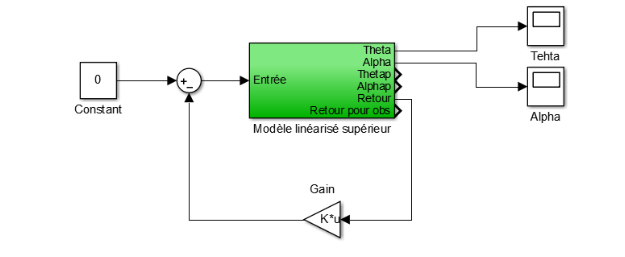
\includegraphics[scale=0.6]{simdispol.png}
\captionof{figure}{\textit{Simulateur du dispositif Linéaire}}
\label{simdispol}
\end{center}



     On s’approchant du point d’équilibre on vois que  $\alpha$ et $\theta$ ont un comportement exponentiels qui converge vers 0 a l'infini.\\ 

\begin{center}
{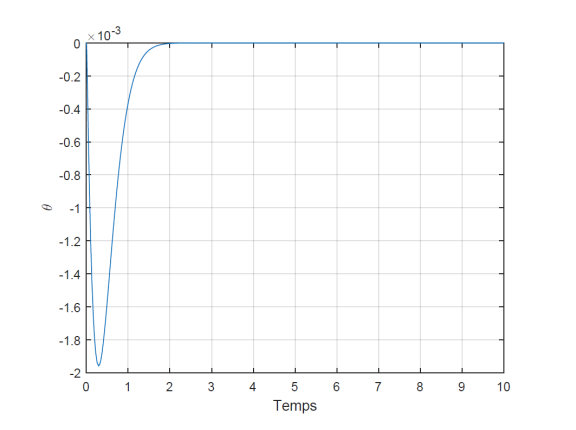
\includegraphics[scale=0.6]{figue1.png}} 
\captionof{figure}{\textit{itsimulation $\alpha$}}
\label{figue1}
\quad

{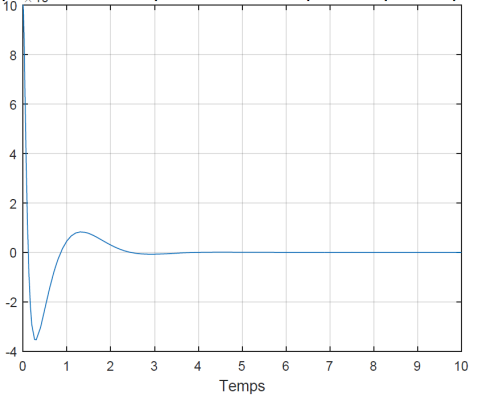
\includegraphics[scale=0.6]{figue2.png}} 
\captionof{figure}{\textit{simulation $\theta$}}
\label{figue2}
\end{center}

    \section{Simuler la réponse aux conditions initiales sur le modèle non linéaire}
   

\begin{center}
{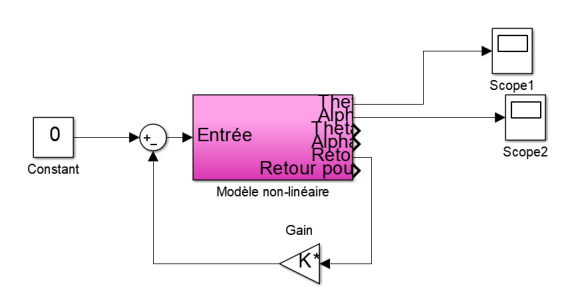
\includegraphics[scale=0.6]{fig3.png}}
\captionof{figure}{\textit{Simulateur du dispositif Non-Linéaire}}
\label{fiig3}
\end{center}

     Autour du point d’équilibre le modèle non linéaire se comporte comme le modèle linéaire.   


\begin{center}
{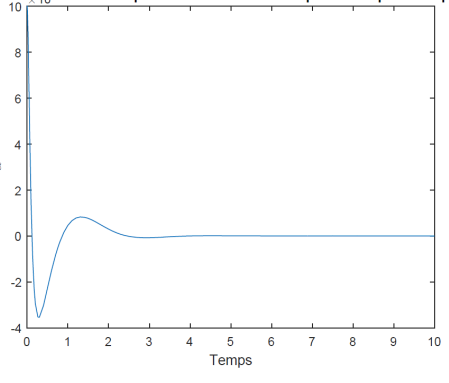
\includegraphics[scale=0.6]{fig4.png}}
\captionof{figure}{\textit{simulation $\alpha$}}
\label{fiig4} 
\end{center}

\begin{center}
{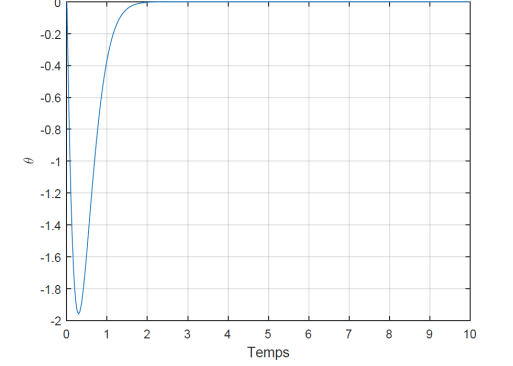
\includegraphics[scale=0.6]{fig5.png}} 
\captionof{figure}{\textit{simulation $\theta$}}
\label{fiig5}
\end{center}


    \section{Étant trop éloignées du point d'équilibre}
     
         Après la simulation du modèle linéaire et non linéaire on remarque que le non linéaire devient instable.\\

\begin{center}
{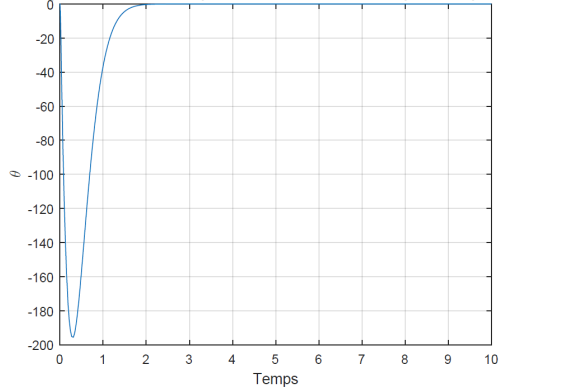
\includegraphics[scale=0.6]{fig6.png}}
\captionof{figure}{\textit{simulation $\alpha$}}
\label{fiig6} 
\quad


{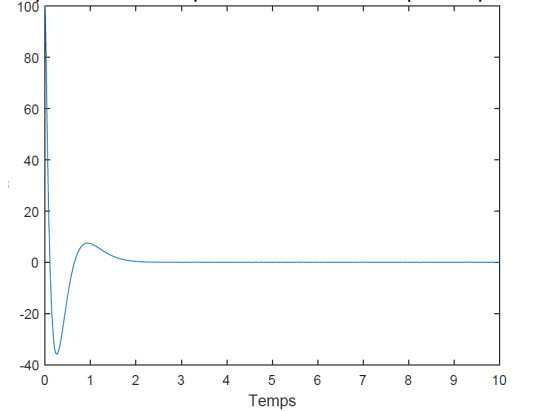
\includegraphics[scale=0.6]{fig7.png}}
\captionof{figure}{\textit{simulation $\theta$}}
\label{fiig7}
\end{center}  

\begin{center}
{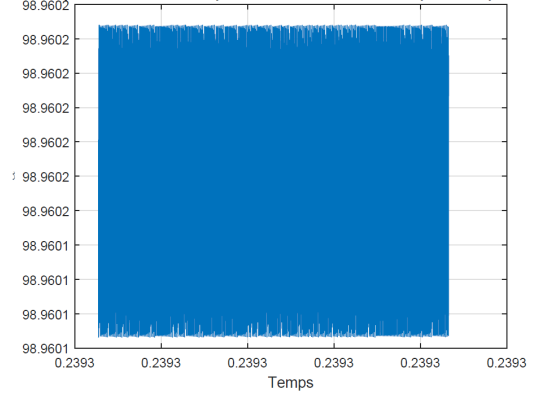
\includegraphics[scale=0.6]{fig8.png}} 
\captionof{figure}{\textit{simulation $\alpha$}}
\label{fiig8}
\quad
{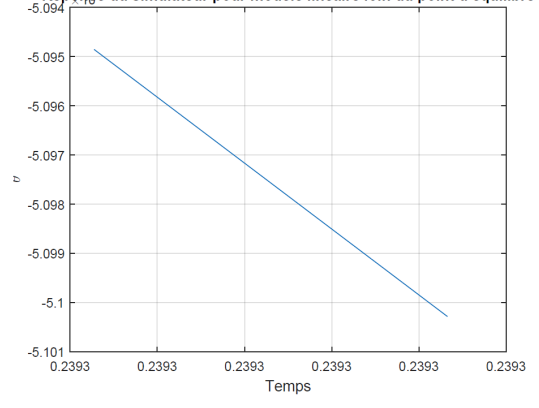
\includegraphics[scale=0.6]{fig9.png}} 
\captionof{figure}{\textit{simulation $\theta$}}
\label{fiig9}
\end{center}


    \section{Vue par l'observateur}

\begin{center}
{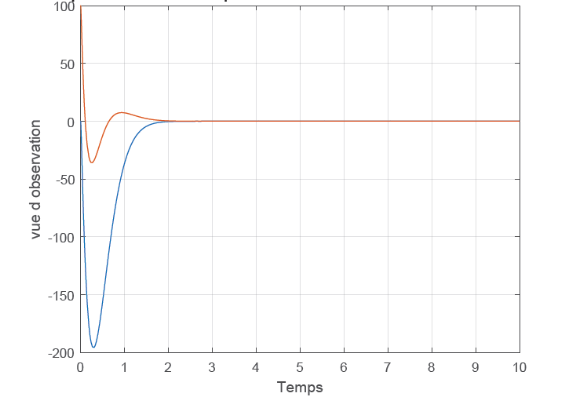
\includegraphics[scale=0.6]{fig10.png}} 
\captionof{figure}{\textit{simulation vue par l'observateur}}
\label{fiig10}
\end{center} 

Remarque: le système est stable asymptotique.

\chapter{IMPLANTATION LOI DE COMMANDE SUR LE DISPOSITIF RÉEL}
     
     Nous constatons que les valeurs après simulation et  
    $K_{haut}$=
$$
\begin{matrix}
-4.4472 &  36.9886  & -3.3994 &   5.3447
\end{matrix} 
$$     

     On va généré grâce à la commande $acker(A_{haut},B_{haut},p)$
pour les pôles $p$=
$$
\begin{matrix}
-108&-0.3&-4.3+2.2i&-4.3-2.2i
\end{matrix}^{T}
$$

     Qui va nous permettre  de stabiliser asymptotiquement $\alpha$ à la valeur final nul tandis que $\theta$ pressente des erreurs car elle n'est pas  stable au point  0.
     
\chapter{APPROCHE ROBUSTE: COMMANDE INTÉGRALE}
     En premier lieux on suppose que les perturbation causé par le système en boucle fermer comme des perturbation constante qui agissent sur la sortie de $\theta$ voir la figure ci-dessous.  
     

\begin{center}
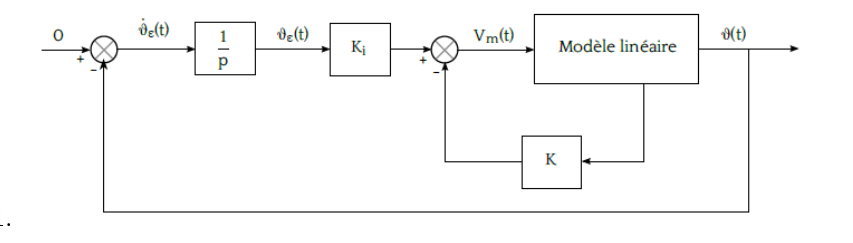
\includegraphics[scale=0.5]{fig11.png} 
\captionof{figure}{\textit{Retour d’état avec commande intégrale}}
\label{fiig11}
\end{center}   

    \section{Représentation d'état du système} 
     
     \begin{equation*}
    \left\{\begin{matrix}
    \dot{x}(t)=Ax(t)+Bu(t)\\ 
    \dot{x_{i}}(t)=Y_{c}-Cx(t)\\
    y(t)=Cx(t)\\
    u(t)=Kx(t)+k_{i}x_{i}(t)
    \end{matrix}\right.
    \end{equation*}
    
    \begin{equation}
    \binom{\dot{x}}{\dot{x_{i}}}=\begin{bmatrix}
    A & 0\\ 
    -C & 0 
    \end{bmatrix}\binom{x}{x_{i}}+\begin{bmatrix}
    B &0 \\ 
    0 & 1
    \end{bmatrix}\binom{U}{Y_{c}}
    \end{equation}
    
    \begin{equation*}
    U=[K  \; K_{i}] \binom{x}{x_{i}}\\
\end{equation*}


\begin{equation*}
\Rightarrow\binom{\dot{x}}{\dot{x_{i}}}=\begin{bmatrix}
A & 0\\ 
-C & 0 
\end{bmatrix}\binom{x}{x_{i}}+\begin{bmatrix}
BK & BK_{i}\\ 
 0& 0
\end{bmatrix}\binom{x}{x_{i}}+ \binom{0}{1}\begin{bmatrix}
Y_{c}
\end{bmatrix}
\end{equation*}


le nouveau vecteur d'état\\

 
 $x_{int}$=
$$ 
 \begin{matrix}
\theta(t) & \alpha(t)& \dot{\theta}(t) & \dot{\alpha}(t)&\theta_{\epsilon}(t) 
\end{matrix}^{T}
 $$
\\

$A_{int}$ =
$$
\begin{matrix}
 0&0&1&0&0\\
 0&0&0&1&0\\
 0&81.4033&-28.8249&-0.9319&0\\
 0&122.0545&-27.7372&-1.3972&0\\
 -1&0&0&0&0
\end{matrix}
$$

$B_{int}$ =
$$
\begin{matrix}
        0\\
         0\\
   51.8323\\
   49.8764\\
         0
\end{matrix}
$$
\quad\quad\quad\
$C_{int}$ =
$$
\begin{matrix}
     1&0&0&0&0\\
     0&1&0&0&0
\end{matrix}
$$
\quad\quad
$D_{int}$=
$$
\begin{matrix}
0\\
0
\end{matrix}
$$

    \section{Calcul de K\{int\}}
    
    Pour les pôles $p\{int\}$=
    $$\begin{matrix}
-108&-4.3+2.25i&-4.3-2.25i&-0.4+0.35i&-0.4-0.35i
\end{matrix}^{T}$$

  La commande $acker(Aint,Bint,pi)$ qui nous as permet d'avoir les valeurs de 
 
 $K\{int\}$=
 $$\begin{matrix}
-1.0203  & 25.2537 &  -2.0482  &  3.8764  &  0.3171
\end{matrix}$$
ces valeurs de $K\{int\}$ on permis de corriger l'erreur de position de $\theta$ et l'annule. 


\chapter{MONTÉE DU PENDULE}
      Pour avoir un modèle linéarisé au point bas un modèle de valeur très oscillant, on utilisant des pôles imaginaire et a partie réelles négatives.   
      
      
      % *********************** Conclusion ***************** 
\chapter*{Conclusion}
	\addcontentsline{toc}{chapter}{Conclusion}
      Suit a ce TP on vue que ce modèle non linéaire soit stable que autour du pont d'équilibre,ce que engendre l'instabilité on s’éloignant de ce point, mais pour le modèle linéaire est stable quelque soit le point choisit.
      Ce TP nous permet la compréhension l’influence du point d’équilibre par apport aux modèle linéaire ou pas.
      Ce que il nous a permet aussi de comprendre l'utilité de la robustesse pour assurée la stabilités des système.   








\begin{appendices}
\chapter*{Annexe 1}
	\addcontentsline{toc}{chapter}{Annexe 1}		
		Voici le code...\hyperref[annexe1]{Retour vers Section 1.1}\label{section1.1}
		
		\begin{lstlisting}
			%Reglage de Te et de l'initialisation
    			Te=0.02;
    			Theta_init=0;
    			Alpha_init_nl=-1;%Origine en haut
    			Alpha_init_sup=0;%Origine en haut
    			Alpha_init_inf=0;%Origine en bas    			
		\end{lstlisting}
		%\hyperref[sec:hello]{Retour vers Section 1.1}
		.\\\\\\
		Voici le code...\hyperref[annexe1]{Retour vers Section 1.1}\label{section1.1}
		\begin{lstlisting}
			%Appel des fichiers
			Espace_etat_ABCD; % A COMPLETER genere {A,B,C,D}{up,int,down}
			systeme_haut = ss(Aup,Bup,Cup,Dup)
			poles_de_Aup = eig(Aup) %1ere question
			commandablite_de_haut = ctrb(Aup,Bup) %2eme question
			rang_com_haut = rank(commandablite_de_haut)%2eme question
			observabilite_de_haut = obsv(Aup,Cup)%3eme question
			rang_obs_haut = rank(observabilite_de_haut)%3eme question		    			
		\end{lstlisting}
		.\\\\\\
		Voici le code...\hyperref[annexe1]{Retour vers Section 1.1}\label{section1.1}
		\begin{lstlisting}
			%%Chapitre 5
			K =  acker(Aup,Bup,[-108 -0.3 -4.3+2.2*i -4.3-2.2*i])
			%     eig(Aup-Bup*K)	   			
		\end{lstlisting}
		.\\\\\\
		Voici le code...\hyperref[annexe1]{Retour vers Section 1.1}\label{section1.1}
		\begin{lstlisting}
			%%Chapitre6
			Te=0.02;
    			Theta_init=25;
    			Alpha_init_nl=0.06;%Origine en haut
    			Alpha_init_sup=3;%Origine en haut
    			Alpha_init_inf=0;%Origine en bas			
		\end{lstlisting}
				
\end{appendices}





%Bibliographie 
%\bibliographystyle{alpha}
%\bibliography{biblio}




\end{document}





